% chapter3.tex -- Generating All Triangulations of a Cycle (Baseline Algorithm)
% Based on the author's UGThesis.docx and Parvez et al. 2011.

\chapter{Generating All Triangulations of a Cycle}
\label{ch:cycle_algorithm}

In this chapter we present the algorithm for generating all triangulations of a cycle with labeled vertices. 
This algorithm, due to Parvez, Rahman, and Nakano~\cite{parvez2011}, forms the core building block of our method for biconnected graphs. 
We describe it in detail, including the necessary definitions, the parent‑child relationship, the data structures, and the complexity analysis.

\section{Problem Definition}
\label{sec:cycle_problem}

Let \(C = \langle v_1, v_2, \dots, v_n \rangle\) be a cycle with \(n\) vertices listed in counterclockwise order. 
All vertices are labeled, and the embedding is fixed. 
A \textbf{triangulation} of \(C\) is a maximal set of non‑crossing chords that partition the interior of \(C\) into triangles. 
Any triangulation contains exactly \(n-3\) chords.

We wish to generate \emph{all} triangulations of \(C\) without duplication, using \(O(1)\) amortized time per triangulation and \(O(n)\) space.

\section{Root Vertex and Root Triangulation}
\label{sec:root_vertex}

We fix an arbitrary vertex as the \textbf{root vertex}. 
In this chapter we take \(v_1\) as the root without loss of generality. 
The \textbf{root triangulation} \(T_r\) is the fan triangulation obtained by connecting \(v_1\) to every other vertex except its neighbours \(v_2\) and \(v_n\) (see Figure~\ref{fig:fan_triangulation}). 
Thus \(T_r\) contains the chords \((v_1, v_3), (v_1, v_4), \dots, (v_1, v_{n-1})\).

\begin{figure}[htbp]
    \centering
    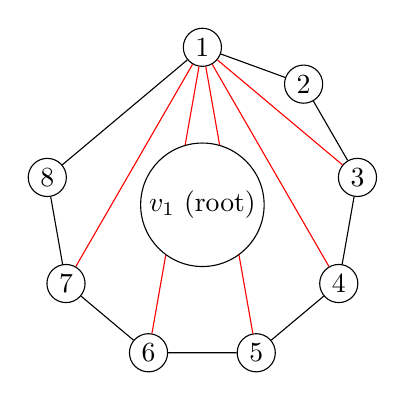
\begin{tikzpicture}[scale=1, every node/.style={circle, draw, fill=white, inner sep=2pt}]
        \foreach \i/\angle in {1/90,2/50,3/10,4/-30,5/-70,6/-110,7/-150,8/170} {
            \node (v\i) at (\angle:2) {\i};
        }
        \draw (v1)--(v2)--(v3)--(v4)--(v5)--(v6)--(v7)--(v8)--(v1);
        \draw[red] (v1)--(v3);
        \draw[red] (v1)--(v4);
        \draw[red] (v1)--(v5);
        \draw[red] (v1)--(v6);
        \draw[red] (v1)--(v7);
        \node at (0,0) {\(v_1\) (root)};
    \end{tikzpicture}
    \caption{Root triangulation (fan) of an octagon. All chords are incident to the root vertex \(v_1\).}
    \label{fig:fan_triangulation}
\end{figure}

In the root triangulation, every vertex except \(v_2\) and \(v_n\) is directly visible from \(v_1\) via a chord. 
We say that \(v_1\) has \textbf{full vision} in \(T_r\).

\section{Visibility and Blocking Chords}
\label{sec:visibility_blocking}

In a general triangulation \(T\) of \(C\), some vertices may be hidden from \(v_1\) by chords that do not involve \(v_1\). 
These chords are called \textbf{blocking chords}.

\begin{definition}[Visible vertex]
    A vertex \(v_j\) is \textbf{visible} from the root \(v_1\) in a triangulation \(T\) if the chord \((v_1, v_j)\) belongs to \(T\).
\end{definition}

\begin{definition}[Blocking chord]
    A chord \((v_i, v_j)\) with \(i, j \neq 1\) is called a \textbf{blocking chord} if the triangle \((v_1, v_i, v_j)\) is present in \(T\). 
    In other words, both \(v_i\) and \(v_j\) are visible from \(v_1\), but the chord \((v_i, v_j)\) blocks the view to vertices between \(v_i\) and \(v_j\) on the cycle.
\end{definition}

\begin{figure}[htbp]
    \centering
    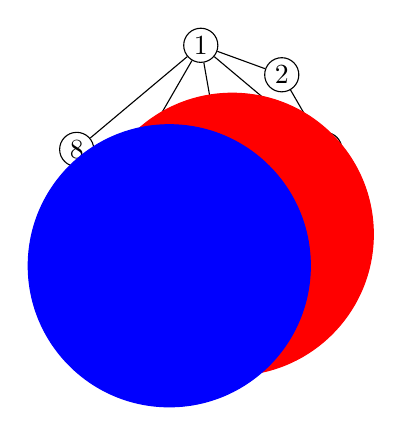
\begin{tikzpicture}[scale=0.8, every node/.style={circle, draw, fill=white, inner sep=1.5pt}]
        \foreach \i/\angle in {1/90,2/50,3/10,4/-30,5/-70,6/-110,7/-150,8/170} {
            \node (v\i) at (\angle:2) {\i};
        }
        \draw (v1)--(v2)--(v3)--(v4)--(v5)--(v6)--(v7)--(v8)--(v1);
        \draw (v1)--(v3);
        \draw (v1)--(v5);
        \draw (v1)--(v7);
        \draw[red, thick] (v3)--(v5);
        \draw[blue, thick] (v5)--(v7);
        \node at (0,0) {\(v_1\)};
        \node[red] at (0.5, -1) {blocking chord \((v_3, v_5)\)};
        \node[blue] at (-0.5, -1.5) {blocking chord \((v_5, v_7)\)};
    \end{tikzpicture}
    \caption{Blocking chords in a triangulation. The chords \((v_3, v_5)\) and \((v_5, v_7)\) block the view from \(v_1\) to vertices \(v_4\) and \(v_6\) respectively.}
    \label{fig:blocking_chords}
\end{figure}

Observe that in the root triangulation there are no blocking chords. 
As we move away from the root, blocking chords appear and reduce the number of vertices visible from \(v_1\).

\section{The Leftmost Blocking Chord}
\label{sec:leftmost_blocking_cycle}

Among all blocking chords of a triangulation \(T\), we select a canonical one to define the parent.

\begin{definition}[Leftmost blocking chord]
    \label{def:leftmost_blocking_cycle}
    Let \((v_b, v_{b'})\) with \(b < b'\) be a blocking chord of \(T\). 
    It is the \textbf{leftmost blocking chord} if no other blocking chord \((v_i, v_j)\) satisfies \(j < b'\). 
    In other words, it has the smallest possible larger endpoint.
\end{definition}

\begin{lemma}[Uniqueness]
    Any triangulation \(T\) that is not the root has exactly one leftmost blocking chord.
\end{lemma}

The proof was given in Chapter~\ref{ch:preliminaries} (Lemma~\ref{lem:unique_leftmost}).

\section{Parent-Child Relationship}
\label{sec:parent_child_cycle}

The genealogical tree \(\mathcal{T}(C)\) is defined by the following parent function.

\begin{definition}[Parent of a triangulation]
    For a non‑root triangulation \(T\), let \((v_b, v_{b'})\) be its leftmost blocking chord. 
    The \textbf{parent} \(P(T)\) is obtained by flipping \((v_b, v_{b'})\) in the quadrilateral that contains it.
\end{definition}

Flipping a blocking chord removes it and adds a chord incident to the root, thereby increasing the number of visible vertices. 
Hence the parent has a clearer view from \(v_1\) than the child.

\begin{lemma}
    Every triangulation \(T \neq T_r\) has a unique parent, and the parent has exactly one more chord incident to \(v_1\) than \(T\).
\end{lemma}

\begin{proof}
    Uniqueness follows from the uniqueness of the leftmost blocking chord. 
    Flipping \((v_b, v_{b'})\) replaces it with a chord \((v_1, v_k)\) for some \(k\) (the opposite vertex of the quadrilateral). 
    Thus the number of chords incident to \(v_1\) increases by one.
\end{proof}

Conversely, a triangulation \(T\) can have several children. 
Each child is obtained by flipping a \textbf{generating chord} of \(T\).

\section{Generating Chords}
\label{sec:generating_chords_cycle}

Let \((v_b, v_{b'})\) be the leftmost blocking chord of \(T\) (if \(T\) is the root, we set \(b = n\) and \(b' = n+1\) for convenience). 
A chord \((v_1, v_j)\) is called a \textbf{generating chord} of \(T\) if flipping it produces a new triangulation whose leftmost blocking chord is exactly the newly added chord.

\begin{lemma}[Condition for generating chords]
    A chord \((v_1, v_j)\) is generating if and only if \(j \ge b'\) (where \(b'\) is the larger endpoint of the leftmost blocking chord, or \(j \ge 3\) for the root).
\end{lemma}

\begin{proof}
    The original proof from Parvez et al.~\cite{parvez2011} uses a case analysis. 
    If \(j < b'\), flipping \((v_1, v_j)\) produces a new chord \((v_p, v_q)\) with \(q \le b'\), so the leftmost blocking chord of the child is still \((v_b, v_{b'})\) (or another chord with the same larger endpoint), and the flipped chord is not the leftmost. 
    Therefore the parent of the child would not be \(T\), so \((v_1, v_j)\) is not generating.

    If \(j \ge b'\), flipping \((v_1, v_j)\) creates a chord \((v_p, v_q)\) with \(q > b'\). 
    One can verify that this new chord becomes the leftmost blocking chord of the child, and \(T\) is its parent. 
    Hence \((v_1, v_j)\) is generating.
\end{proof}

\begin{figure}[htbp]
    \centering
    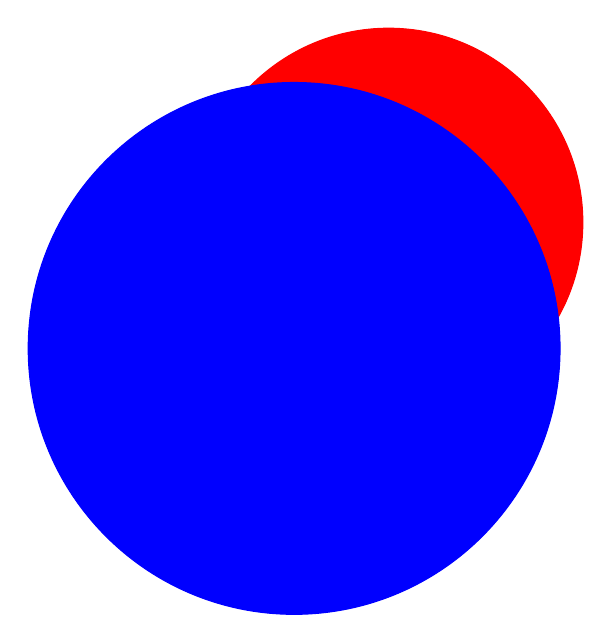
\begin{tikzpicture}[scale=0.8, every node/.style={circle, draw, fill=white, inner sep=1.5pt}]
        \foreach \i/\angle in {1/90,2/60,3/30,4/0,5/-30,6/-60,7/-90,8/-120,9/-150,10/180} {
            \node (v\i) at (\angle:2) {\i};
        }
        \draw (v1)--(v2)--(v3)--(v4)--(v5)--(v6)--(v7)--(v8)--(v9)--(v10)--(v1);
        \draw (v1)--(v4);
        \draw (v1)--(v6);
        \draw (v1)--(v8);
        \draw[red, thick] (v4)--(v6);
        \draw[blue, thick] (v6)--(v8);
        \node at (0,0) {\(v_1\)};
        \node[red] at (1.5, 0.5) {leftmost blocking chord \((v_4, v_6)\)};
        \node[blue] at (0, -1.5) {generating chords: \((v_1, v_6)\), \((v_1, v_8)\), \((v_1, v_9)\)};
    \end{tikzpicture}
    \caption{Generating chords in a triangulation. The leftmost blocking chord is \((v_4, v_6)\); therefore the generating chords are those with \(j \ge 6\): \((v_1, v_6)\), \((v_1, v_8)\), \((v_1, v_9)\).}
    \label{fig:generating_chords}
\end{figure}

The root triangulation has no blocking chord; by convention we set \(b' = 3\), so all chords \((v_1, v_j)\) with \(j = 3,4,\dots,n-1\) are generating. 
Thus the root has \(n-3\) children.

\section{Data Structures}
\label{sec:data_structures_cycle}

To represent a triangulation \(T\) of \(C\) and to generate its children efficiently, we maintain three lists:

\begin{itemize}
    \item \textbf{\(L\) (chord list)}: The set of all chords of \(T\), stored in a linked list.
    \item \textbf{\(GS\) (generating set)}: The list of generating chords of \(T\). 
    For the root, \(GS = L\).
    \item \textbf{\(O\) (opposite pairs)}: For each generating chord \((v_1, v_j)\), we store its \textbf{opposite pair} \((v_o, v_{o'})\) where \(o < j < o'\) and the quadrilateral \((v_1, v_o, v_j, v_{o'})\) is present in \(T\). 
    Flipping \((v_1, v_j)\) replaces it with \((v_o, v_{o'})\).
\end{itemize}

All three lists require \(O(n)\) space because a triangulation of \(n\) vertices has exactly \(n-3\) chords.

\section{Algorithm for Generating All Triangulations of a Cycle}
\label{sec:cycle_algorithm_pseudocode}

We now present the algorithm in pseudocode. 
The main procedure is a depth‑first traversal of the genealogical tree \(\mathcal{T}(C)\).

\begin{algorithm}[htbp]
    \caption{GenerateAllTriangulationsCycle}
    \label{alg:cycle_main}
    \begin{algorithmic}[1]
        \Procedure{GenerateAllTriangulationsCycle}{$C$}
            \State $v_r \gets v_1$ \Comment{Choose root vertex}
            \State $T_r \gets$ \Call{BuildRootTriangulation}{$C, v_r$}
            \State \Call{Output}{$T_r$}
            \State \Call{DFS}{$T_r$}
        \EndProcedure
    \end{algorithmic}
\end{algorithm}

\begin{algorithm}[htbp]
    \caption{BuildRootTriangulation}
    \label{alg:build_root}
    \begin{algorithmic}[1]
        \Procedure{BuildRootTriangulation}{$C, v_r$}
            \State $L \gets \emptyset$, $GS \gets \emptyset$, $O \gets \emptyset$
            \For{$j = 3$ \textbf{to} $n-1$}
                \State Add chord $(v_r, v_j)$ to $L$ and $GS$
                \State Store opposite pair $(v_{j-1}, v_{j+1})$ for $(v_r, v_j)$ in $O$
            \EndFor
            \State \Return $(L, GS, O)$
        \EndProcedure
    \end{algorithmic}
\end{algorithm}

\begin{algorithm}[htbp]
    \caption{DFS (Depth‑first traversal of \(\mathcal{T}(C)\))}
    \label{alg:dfs_cycle}
    \begin{algorithmic}[1]
        \Procedure{DFS}{$T$}
            \State Let $(v_b, v_{b'})$ be the leftmost blocking chord of $T$ \Comment{If none, set $b' = 3$}
            \For{each generating chord $(v_1, v_j) \in GS$ with $j \ge b'$}
                \State $T' \gets$ \Call{Flip}{$T, (v_1, v_j)$}
                \State \Call{Output}{$T'$}
                \State \Call{DFS}{$T'$}
            \EndFor
        \EndProcedure
    \end{algorithmic}
\end{algorithm}

The flip operation (Algorithm~\ref{alg:flip_cycle}) creates a child triangulation in constant time by updating the three lists.

\begin{algorithm}[htbp]
    \caption{Flip}
    \label{alg:flip_cycle}
    \begin{algorithmic}[1]
        \Procedure{Flip}{$T, (v_1, v_j)$}
            \State Find opposite pair $(v_o, v_{o'})$ from $O$ for $(v_1, v_j)$
            \State Remove $(v_1, v_j)$ from $L$ and $GS$
            \State Add $(v_o, v_{o'})$ to $L$ (but not to $GS$)
            \State Update opposite pairs of the two neighbouring generating chords $(v_1, v_{o})$ and $(v_1, v_{o'})$ (if they exist)
            \State Recompute $GS$ for the new triangulation (only chords with $j \ge$ new leftmost blocking chord remain generating)
            \State \Return the new triangulation $T'$
        \EndProcedure
    \end{algorithmic}
\end{algorithm}

\begin{remark}
    Updating the opposite pairs affects at most two chords (the neighbours of the flipped chord). 
    Therefore the entire flip operation takes \(O(1)\) time.
\end{remark}

\section{Correctness}
\label{sec:cycle_correctness}

The algorithm correctly generates all triangulations without duplicates because:

\begin{enumerate}
    \item The parent of any non‑root triangulation is uniquely defined (by the leftmost blocking chord). 
    Hence each triangulation appears exactly once in the tree, and the DFS visits each node exactly once.
    \item The generating chords are exactly those whose flips produce children that are valid and have the current triangulation as parent (Lemma~\ref{lem:generating_condition} in the original paper). 
    Thus no child is missed.
    \item The recursion terminates because the depth is bounded by the number of chords incident to \(v_1\), which is at most \(n-3\).
\end{enumerate}

\section{Time and Space Complexity}
\label{sec:cycle_complexity}

\subsection{Time Complexity}

Building the root triangulation takes \(O(n)\) time (adding \(n-3\) chords and initialising the lists). 
For each edge flip (generating a child from a parent), we perform a constant number of operations: 
removing one chord, adding another, and updating at most two opposite pairs. 
Thus each child is generated in \(O(1)\) time.

Let \(T\) be the total number of triangulations of \(C\). 
The number of edges in the genealogical tree is \(T - 1\) (one parent edge per non‑root node). 
Since the DFS traverses each edge once, the total number of flip operations is \(T - 1\). 
Hence the total time is \(O(n + T) = O(T)\) (because \(n = O(T)\) when \(n \ge 4\), as Catalan numbers grow exponentially). 
Therefore the amortised time per triangulation is \(O(1)\).

\subsection{Space Complexity}

At any point during the DFS, we store:
\begin{itemize}
    \item The lists \(L, GS, O\) for the current triangulation: \(O(n)\).
    \item The recursion stack: depth at most \(n-2\) (each flip increases the number of chords incident to \(v_1\) by one, starting from 0 at the root and reaching at most \(n-3\) at leaves). 
    Hence stack size is \(O(n)\).
\end{itemize}
No other storage is required because we do not keep the entire tree in memory. 
Thus the space complexity is \(O(n)\).

\section{Example: Triangulations of a Hexagon}
\label{sec:hexagon_example}

Figure~\ref{fig:hexagon_tree} shows the genealogical tree for a hexagon (\(n=6\)). 
The root has \(n-3 = 3\) generating chords, leading to three children. 
Each child may have fewer generating chords, and the depth is at most 4 (including the root). 
The total number of triangulations of a convex hexagon is 14, which matches the Catalan number \(C_4 = 14\).

\begin{figure}[htbp]
    \centering
    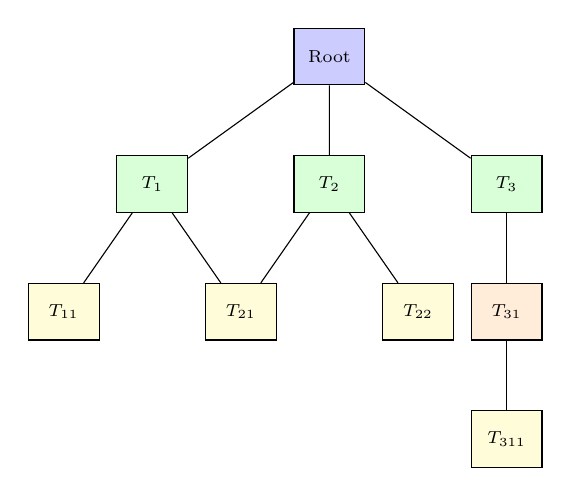
\begin{tikzpicture}[level distance=1.8cm, sibling distance=2.5cm, scale=0.9, transform shape]
        \tikzset{every node/.style={rectangle, draw, minimum width=1cm, minimum height=0.8cm, align=center, font=\scriptsize}}
        \node[fill=blue!20] {Root}
            child { node[fill=green!15] {$T_1$}
                child { node[fill=yellow!15] {$T_{11}$} }
                child { node[fill=yellow!15] {$T_{12}$} }
            }
            child { node[fill=green!15] {$T_2$}
                child { node[fill=yellow!15] {$T_{21}$} }
                child { node[fill=yellow!15] {$T_{22}$} }
            }
            child { node[fill=green!15] {$T_3$}
                child { node[fill=orange!15] {$T_{31}$}
                    child { node[fill=yellow!15] {$T_{311}$} }
                }
            };
    \end{tikzpicture}
    \caption{Genealogical tree for a hexagon. The root has three children; the total number of nodes is 14.}
    \label{fig:hexagon_tree}
\end{figure}

\section{Summary}
\label{sec:cycle_summary}

We have described the Parvez–Rahman–Nakano algorithm for generating all triangulations of a labeled cycle. 
Key properties:
\begin{itemize}
    \item The genealogical tree is traversed in depth‑first order.
    \item Each child is generated from its parent by flipping a generating chord in \(O(1)\) time.
    \item The space complexity is \(O(n)\).
    \item The amortised time per triangulation is \(O(1)\).
\end{itemize}

This algorithm is used as a subroutine in our method for biconnected plane graphs, where we process each face independently while maintaining a global set of chords to avoid multi‑edges.